\chapter{Game Engines}\label{ch:gameengines}
Eine \textit{Game Engine} ist ein komplexes Software-Framework, das für die Erstellung, Entwicklung und Bereitstellung interaktiver digitaler Anwendungen konzipiert ist, vor allem für Videospiele, aber auch für Simulationen, Architekturvisualisierungen und vieles mehr. Dabei ist das Hauptziel einer Game Engine, eine Abstraktion der allgemeinen Videospielfunktionen anzubieten, damit Code und Spielkomponente in verschiedenen Projekten wiederverwendet werden können. Die Funktionen einer modernen Game Engine können eine Rendering-Engine für 2D- oder 3D-Grafiken, Handhabung von Inputs, Physik-Engine, Animationen, Speichermanagement und Prozess-Threading sein. Bei vielen modernen Game Engines verwenden Entwickler höhere Programmiersprachen, wie Java, \cpp{} und \csharp{}, zum Entwickeln der Skripte für die Spiele.\cite{appacademyBestProgramming} Außerdem werden immer mehr Plattformen angeboten, für welche die Spiele entwickelt werden können, sei es für Desktop-Umgebungen, Mobilgeräte oder Konsolen.\cite{andrade2015game}

In diesem Kapitel werden drei Game Engines genauer betrachtet. Es wird die populäre Game Engine Unity\cite{vsmid2017comparison}, die von Epic Games veröffentlichte Unreal Engine und die neuere Godot Engine untersucht. Alle Game Engines bieten eine Vielzahl von Möglichkeiten an, den Spielstand von einem Spieler abzuspeichern und zu laden. Teilweise gibt es auch bereits fertige Speicher- und Ladesysteme, die als Entwickler verwendet werden können.
%--------------------------------------------------------------------------



%--------------------------------------------------------------------------
\section{Unity}
\textit{Unity} ist eine leistungsstarke und vielseitige Echtzeit-3D-Entwicklungsplattform zum Entwickeln von Videospielen und Filmen. Sie wurde 2005 von Unity Technologies entwickelt und durch die intuitive Benutzeroberfläche schnell zu der meist-verwendeten Game Engine der Welt. Unity bietet für Spieleentwickler eine breite Auswahl an Systemen an, für das Programmieren von 2D- und 3D-Spielen, Simulationen oder interaktiven Anwendungen. Es ist möglich, Unity für Mobilspiele, verschiedene Betriebssysteme, wie Windows, MacOS oder Linux, oder Spiele für Konsolen zu entwickeln. Programmiert wird bei Unity hauptsächlich mit der Programmiersprache \csharp{}.\cite{unityUnityEngine}\cite{vsmid2017comparison}

In diesem Kapitel wird eine Vielzahl von Möglichkeiten angeschaut, welche Unity anbietet, um Speicher- und Ladesysteme für das Speichern des Spielstandes aufzustellen. Als Erstes wird Unitys PlayerPrefs-Klasse angeschaut. Danach werden verschiedene Arten aufgezählt, Objekte von Unity in \ac{json} zu serialisieren und wann welche Strategie sinnvoll ist. Anschließend werden die .NET-Klassen BinaryFormatter, StreamWriter und StreamReader betrachtet. Beim BinaryFormatter werden die Probleme beim Serialisieren und Deserialisieren von Daten erläutert und es werden Alternativen vorgestellt. Abschließend wird das kostenpflichtige Paket Easy Save aus dem Asset Store angeschaut, welches einfach und effizient ein komplettes Speicher- und Ladesystem für Spiele implementieren kann.



\subsection{PlayerPrefs}
Bei Speicher- und Ladesystemen bietet Unity für Entwickler wenige eingebaute Funktionen. Jedoch gibt es die PlayerPrefs, welche eine einfache Art ist Daten zu speichern, aber ist dabei auch sehr limitiert. PlayerPrefs, was für Player Preferences steht, ist eigentlich zum Speichern von Konfigurationen, wie die Auflösung oder Lautstärke des Spieles gedacht. Jedoch lassen sich damit jede Art von Informationen speichern. Das Speichern wird mit Funktionen der PlayerPrefs-Klasse gemacht, wobei nur die Datentypen string, float und integer unterstützt werden. Über einen Schlüssel lässt sich dann ein Schlüsselwert dieser Datentypen festlegen oder es kann dieser erhalten werden. Die Werte der PlayerPrefs-Klasse werden mit der klasseninternen Save-Funktion gespeichert. Diese kann während der Laufzeit im Code aufgerufen werden und wird automatisch bei der Terminierung des Spieles aufgerufen.\cite{unityPlayerPrefsSave} Je nach Betriebssystem werden die PlayerPrefs in einem unterschiedlichen Dateiformat abgespeichert, die Daten werden aber nicht verschlüsselt.\cite{unityPlayerPrefs}

Allgemein wird davon abgeraten, Unitys PlayerPrefs-System für das Speichern des Spielstandes zu verwenden.\cite{unityPersistentData}\cite{logrocketPlayerPrefs}\cite{gamedevbeginnerPlayerPrefs} Zum einen werden die Daten eines Spieles alle am selben Ort abgespeichert. Wenn es aber in dem Spiel verschiedene Spielstände geben soll, gibt es bereits Probleme mit diesem Ansatz. Eine mögliche Lösung von diesem Problem wäre es, dass jeder Spielstand eine Identifikationsnummer bekommt, welche dann an jedem Schlüssel hinzugefügt wird.\cite{logrocketPlayerPrefs} Die ganzen Identifikationsnummern müssen aber auch gespeichert werden, wo auch schon das nächste Problem mit PlayerPrefs auftritt. Es gibt wenige verfügbare Datentypen, die verwendet werden können. Wenn zum Beispiel eine Liste der Identifikationsnummern aller Spielstände gespeichert werden soll, kann dies nicht ohne größeren Aufwand gemacht werden.\cite{logrocketPlayerPrefs} Über den string-Datentyp lassen sich jedoch \ac{json}-Strings speichern, wodurch wieder mehr Datentypen, wie Listen und andere Gruppierungen von Daten, möglich sind. Wie auch schon erwähnt, ist die PlayerPrefs-Klasse zum Speichern von Konfigurationen gedacht, nicht zum Speichern des Spielstandes. Bei Windows werden die PlayerPrefs in der Registry abgespeichert. Die Registry, oder auch Windows-Registrierungsdatenbank genannt, ist zum Speichern von Konfigurationen des Systems und von Anwendungen.\cite{logrocketPlayerPrefs} Bei größeren Datenmengen könnte dieses System sehr langsam werden.\cite{gamedevbeginnerPlayerPrefs}


\subsection{JSON}
Falls viele Daten gespeichert werden sollen und der Aufwand für den Entwickler gering gehalten werden soll, ist \ac{json} eine gute Alternative zu den PlayerPrefs. Auch hier bietet Unity ein Tool namens \textit{JsonUtility} an, welches die \csharp{}-Objekte über Data Binding serialisieren kann. JsonUtility hat zwar einige Einschränkungen, ist dafür aber die schnellste Art, Objekte in \ac{json} zu serialisieren. Eine Einschränkung von JsonUtility ist, dass es einige Typen gibt, die nicht unterstützt werden, wie Dictionary\texttt{<>}, multidimensionale oder Jagged\footnote{Jagged Arrays sind Arrays, dessen Elemente Arrays aus verschiedener Größe sind.\cite{microsoftVerzweigteArrays}} Arrays. Diese lassen sich nicht mit JsonUtility serialisieren. In dem Listing \ref{lst:jsonUtilityExp} werden die drei Funktionen, die JsonUtility anbietet, demonstriert. Von der Zeile 1 bis 7 wird eine Spieler-Klasse definiert, welche dann in einer anderen Klasse, wie ab der Zeile 11 zu sehen ist, verwendet wird. Diese muss mit dem Attribut "Serializable" gekennzeichnet werden, damit diese auch serialisierbar ist. Alle Variablen, die in dieser Klasse public oder mit "[SerializeField]" gekennzeichnet werden, werden beim Serialisierungsprozess betrachtet. Als Erstes werden drei Spieler-Objekte definiert, welche in den Zeilen 15 bis 18 zu \ac{json}-Strings serialisiert werden. In der Zeile 16 ist zu sehen, wie einer der \ac{json}-Strings aussieht. Der Spieler mit dem Namen "Joe" wird dann in den letzten zwei Zeilen zweimal überschrieben. Einmal mit den Werten der Spielerin "Alice" und einmal mit den Werten des Spielers "Tom".\cite{unityJsonUtility}\cite{unitySerializationRules} 

\begin{listing}[htp]
    \begin{minted}{csharp} 
        [Serializable]
        public class Player
        {
            public int level;
            public float health;
            public string name;
        }

        ...
        
        Player joe = new Player() { level = 1, health = 75.2f, name = "Joe" };
        Player alice = new Player() { level = 3, health = 100.0f, name = "Alice" };
        Player tom = new Player() { level = 2, health = 1.0f, name = "Tom" };

        string joeJson = JsonUtility.ToJson(joe);
        //  {"level":1,"health":75.2,"name":"Joe"}
        string aliceJson = JsonUtility.ToJson(alice);
        string tomJson = JsonUtility.ToJson(tom);

        joe = JsonUtility.FromJson<Player>(aliceJson);
        JsonUtility.FromJsonOverwrite(tomJson, joe);
    \end{minted}
    \caption{Serialisieren und Deserialisieren mit JsonUtility}
    \label{lst:jsonUtilityExp}
\end{listing}

Eine populäre Alternative zu JsonUtility ist die \textit{Newtonsoft.JSON}-Bibliothek, auch bekannt als \textit{Json.NET}. Sie wird sehr häufig bei \csharp{}-Projekten verwendet, da sie einfach zu verwenden ist und das Umwandeln zwischen .NET-Objekten und \ac{json} in schnellen Laufzeiten bewältigen kann.\cite{newtonsoftJsonNETNewtonsoft} Der Vorteil gegenüber JsonUtility ist, dass alle nicht serialisierbaren Klassen von JsonUtility mit Json.NET serialisierbar sind. Es ist beispielsweise möglich, ein Dictionary\texttt{<>} zu serialisieren\cite{newtonsoftSerializeDictionary}\cite{newtonsoftDeserializeDictionary} oder jegliche Arten von Arrays. Json.NET wird auch seit der Unity Version 2018.4\footnote{Die Unity Version 2018.4 wurde 2019 veröffentlicht.\cite{unityDownloadArchive}} als Paket unterstützt.\cite{NewtonsoftJsonUnitySupport} Beim Serialisieren von Objekten werden auch bei Json.NET alle Variablen, die public sind, serialisiert. Um beim Serialisieren weniger Daten entstehen zu lassen, bietet Json.NET einige Funktionen an, wie zum Beispiel das Attribut "[JsonIgnore]", mit dem sich Variablen beim Serialisierungsprozess ignorieren lassen, oder die NullValueHandling Einstellung, mit der eingestellt werden kann, ob null-Werte gespeichert werden sollen. Dadurch, dass Json.NET viele Einstellungen anbietet, bei denen der komplette Serialisierungsprozess anpassbar ist, lassen sich die Laufzeiten für Projekte stark optimieren.\cite{newtonsoftReducingSerialized}\cite{newtonsoftPerformanceTips}

Eine weitere .NET-Bibliothek, die verwendet werden kann, ist \textit{LitJSON}. Auch diese ermöglicht es, .NET-Objekte in \ac{json} und umgekehrt zu konvertieren.\cite{litjsonLitJSONDocumentation} LitJSON bietet zwar weniger Funktionen als Json.NET an, aber es ist mithilfe des JsonReader und JsonWriter möglich, über die LitJSON Streaming API zu serialisieren und somit eine eigene Serialisierung der Klassen zu konstruieren.\cite{litjsonLitJSONReaders} Es gibt auch eine Bibliothek, wo LitJSON angepasst wurde, damit die .NET-Bibliothek auch für Unity verwendet werden kann.\cite{githubGitHubMervillUnityLitJson}

Wenn für das Unity-Projekt die Spielstände mit \ac{json} gespeichert werden sollen, stellt sich die Frage, welche Serialisierungs-Klasse oder -Bibliothek sich besser eignet. Wie in der Abbildung \ref{fig:unityJsonPerformance} zu sehen, ist JsonUtility die schnellste Art, Objekte in \ac{json} umzuwandeln und umgekehrt. Die schnellen Laufzeiten von JsonUtility haben auch den Preis, dass die Klasse etwas eingeschränkt ist und einfach gehalten wurde. Sobald es komplexere Datenstrukturen gibt, ist das Arbeiten mit JsonUtility eine große Herausforderung. Da kann sich der Entwickler dann doch für Json.NET oder LitJSON entscheiden, da diese mehr Datentypen unterstützten. Wenn es wichtig ist, dass das Programm schnell serialisiert werden soll, dann ist LitJSON die bessere Wahl zum Arbeiten mit \ac{json}. Falls das Deserialisieren möglichst schnell laufen soll, ist Json.NET geeigneter.

\begin{figure}[htp]
    \centering
    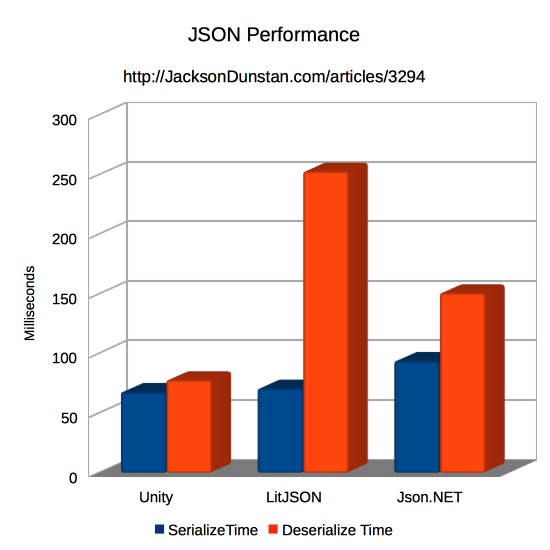
\includegraphics[width=0.6\textwidth]{images/UnityJsonPerformance.png}
    \caption{Laufzeiten der unterschiedlichen \ac{json}-Bibliotheken für Unity bei einer Datenmenge von 101 Bytes \cite{jacksondunstanJacksonDunstancomJSON}}
    \label{fig:unityJsonPerformance}
\end{figure}



\subsection{BinaryFormatter}\label{ssec:binaryFormatter}
Die .NET-Klasse \textit{BinaryFormatter} ist eine Möglichkeit, eine binäre Serialisierung der Daten durchzuführen. Sie verwandelt .NET-Objekte in eine Liste von Bytes um und umgekehrt. In dem Listing \ref{lst:binaryFormatterExp} ist zu sehen, wie der BinaryFormatter verwendet werden kann. Dabei werden die Player-Klasse und die Spieler aus dem Listing \ref{lst:jsonUtilityExp} benutzt. In der Zeile 2 wird der Spieler namens "Joe" in der Datei "joeFile" in binärer Form abgespeichert. In der Zeile 3 wird das Objekt namens "tom" mit den Werten aus der "joeFile"-Datei neu gesetzt. Dabei werden die Daten aus "joeFile" wieder deserialisiert.\cite{microsoftBinaryFormatterClass} 

\begin{listing}[htp]
    \begin{minted}{csharp} 
        BinaryFormatter formatter = new BinaryFormatter();
        formatter.Serialize(joeFile,joe);
        tom = (Player) formatter.Deserialize(joeFile);
    \end{minted}
    \caption{Serialisieren und Deserialisieren der Objekte aus \ref{lst:jsonUtilityExp} mit dem BinaryFormatter}
    \label{lst:binaryFormatterExp}
\end{listing}

Allgemein wird jedoch von dem Verwenden des BinaryFormatters abgeraten. Die Gefahr von Sicherheitsrisiken beim Deserialisieren ist groß. Ein Angreifer könnte den abgespeicherten Binärcode so verändern, dass dieser einen Code im Kontext des Zielprozesses ausführen wird. Je nach Anwendungstyp können solche Angriffe auch zu einem DoS-Angriff\footnote{Bei einem Denial of Service Angriff wird das Zielsystem mit etlichen Anfragen überflutet, was zu einer starken Verlangsamung, bis hin zu einem Zusammenbruch des Systems führen kann.\cite{bundDoSDDoSAttacken}} oder Veröffentlichung von Informationen führen.\cite{microsoftDeserializationRisks}

Eine sicherere Alternative zum BinaryFormatter sind die .NET-Klassen \textit{BinaryReader} und \textit{BinaryWriter}. Diese bieten Funktionalitäten, zum Schreiben von primitiven Datentypen in Binärcode und zum Umwandeln von Binärcode in primitive Datentypen an. Mit dieser Methode ist es zwar aufwendiger, die Daten zu speichern und zu laden, aber dafür sicherer als der BinaryFormatter.\cite{microsoftBinaryReaderClass}\cite{microsoftBinaryWriterClass} 

Ansonsten, wenn die Datenstrukturen komplexer werden, kann der Protocol Buffer aus \ref{sssec:binSerialisierung} verwendet werden. Als Entwickler kann entweder direkt der Protocol Buffer verwendet werden, da dieser auch \csharp{} unterstützt \cite{protobufLanguageGuide}, oder es kann mit Tools gearbeitet werden, die das Kompilieren der Proto-Dateien in Unity übernehmen.\cite{githubProtobufUnity}



\subsection{StreamWriter und StreamReader}
Eine weitere Alternative zu \ac{json} und dem binären Serialisieren der Daten mit Unity sind die .NET-Klassen StreamWriter und StreamReader. Mit dem StreamWriter lassen sich Zeilen in Dateien schreiben und mit dem StreamReader lassen sich diese dann lesen.\cite{microsoftStreamWriterKlasse}\cite{microsoftStreamReaderKlasse} Als Entwickler kann dann entschieden werden, ob Formate wie \ac{json}, Binärcode oder XML verwendet werden, oder ob zum Speichern der Daten ein eigenes Format konzipiert werden soll. Zum Beispiel können einfache Datenstrukturen, wie eine Liste von Identifikationsnummern, Zeile für Zeile in einer eigenen Datei gespeichert werden. Es kann zu Komplikationen kommen, wenn das Format zum Speichern der Daten geändert wird. Die alten Daten müssten dann alle in das neue Format übersetzt werden.



\subsection{Easy Save}
Falls ein Entwickler Zeit sparen will und etwas Budget für das Projekt bereitstellt, kann das \textit{Easy Save} Paket vom Unity Asset Store in Betracht gezogen werden. Dieses Tool bietet ein komplettes Speicher- und Ladesystem für Unity-Projekte an, um eine einfache und effiziente Verwaltung der Daten zu ermöglichen.\cite{unityEasySave} In dem Listing \ref{lst:easySaveExp} ist zu sehen, wie ein Wert in das Speichersystem mit aufgenommen werden kann, indem das Level des Spielers gespeichert und geladen wird. ES3 ist die Klasse von Easy Save und wie zu sehen ist, werden die Daten mit einem Schlüssel-Wert-System gespeichert, ähnlich wie bei einem Dictionary.\cite{moodkieGettingStarted} Easy Save unterstützt viele Datentypen, wie Struct, Array, Dictionary, HashSet oder ganze Components\footnote{Die Basis-Klasse in Unity, die an den Spielobjekten (GameObject-Klasse) hinzugefügt werden kann.\cite{unityComponent}}.\cite{moodkieSupportedTypes} Falls ein Datentyp nicht von Easy Save unterstützt wird, kann mit den ES3Types ganz einfach neue Datentypen zu dem System hinzugefügt werden.\cite{moodkieChoosingWhat} Es ist auch möglich, die gespeicherten Daten zu verschlüsseln oder zu komprimieren.\cite{moodkieGettingStarted} Vorausgesetzt, die Daten sollen automatisch gespeichert werden, kann die "Auto Save"-Funktion von Easy Save verwendet werden.\cite{moodkieAutoSave} Um eine bessere Leistung aus dem Speicher- und Ladesystem herauszuholen, kann mit Easy Save direkt eine Datei zum Speichern der Daten im Cache erstellt werden. Daten, die dann dort gespeichert werden, können während der Laufzeit schneller geladen werden.\cite{moodkieImprovingPerformance} Außerdem lassen sich Strings und Bytes direkt in den Speicherdateien schreiben und lesen.\cite{moodkieSavingLoading} 

\begin{listing}[htp]
    \begin{minted}{csharp} 
        int playerLevel = 1;
        ES3.Save("playerLevel", playerLevel);
        ... 
        if(ES3.KeyExists("playerLevel")) playerLevel = ES3.Load<int>("playerLevel")
    \end{minted}
    \caption{Speichern und Laden eines Integers mit Easy Save}
    \label{lst:easySaveExp}
\end{listing}



\subsection{Strategie für Unity}
Wie zu sehen ist, gibt es verschiedene Herangehensweisen für das Speichern und Laden des Spielstandes mit Unity. Welche Strategie ist für Unity am sinnvollsten? Kurz gesagt gibt es kein System, das in jedem Szenario das vorteilhafteste ist. Welche Strategie verwendet werden sollte, hängt von der Situation ab. 

Wenn Schnelligkeit und Kompaktheit der Daten die oberste Priorität sind, ist die binäre Serialisierung die beste Wahl (siehe \ref{fig:protobufTime} und \ref{fig:protobufBrowser}). Der Protocol Buffer wäre dabei die einfachste Art, dies umzusetzen, vor allem wenn die Datenstrukturen komplexer sind. Es gibt bereits viele Entwickler, die den Protocol Buffer in ihrem Unity-Projekt verwenden, da die \csharp{}-Unterstützung bereits vorhanden ist. 

Falls der Entwickler oder Spieler die gespeicherten Daten lesen und bearbeiten können sollte, ist die Serialisierung zu \ac{json} sinnvoller. Wenn das Spiel zum Beispiel \acp{mod} haben soll, die von individuellen Spielern und Entwicklern erstellt werden können, dann sind Formate wie \ac{json} einfacher zu verstehen. Falls Geschwindigkeit das Wichtigste an dem Projekt ist, ist das JsonUtility-Tool von Unity die beste Wahl (siehe \ref{fig:unityJsonPerformance}). Hier muss jedoch für manche Datenstrukturen eine Serialisierung zu \ac{json} entwickelt werden, was bei komplexen Datenstrukturen sehr aufwendig sein kann. Falls die Zeit lieber gespart werden soll, ist Json.NET oder LitJSON eine gute Alternative. Beide sind im Vergleich zu JsonUtility zwar etwas langsamer, jedoch fällt dies erst bei sehr großen Datenmengen auf. Dadurch, dass beide aber mehr Datenstrukturen unterstützten, kann ein Entwickler bei der Serialisierung mit diesen Tools viel Zeit sparen. Im Durchschnitt ist Json.NET etwas schneller als LitJSON (siehe \ref{fig:unityJsonPerformance}), wenn jedoch schnelle Serialisierungszeiten wichtig sind, dann sollte LitJSON verwendet werden. Dies wäre zum Beispiel vorteilhaft, wenn es viele Serialisierungsprozesse gibt und nur am Anfang des Spieles die Daten deserialisiert werden.  

Ansonsten, wenn der Entwickler möglichst wenig Zeit für das Entwickeln des Speicherns und Ladens des Spielstandes brauchen möchte, ist das Easy Save Paket eine gute Alternative. Dieses bietet auch viele Optimierungsmöglichkeiten an, um das System effizienter laufen zu lassen. Für Unity gibt es auch kostenfreie Speicher- und Ladesysteme, wie zum Beispiel das Component-Save-System\footnote{https://github.com/AlexMeesters/Component-Save-System} von Alex Meesters. 
%--------------------------------------------------------------------------



%--------------------------------------------------------------------------
\section{Unreal Engine}
\textit{Unreal Engine} ist eine von Epic Games entwickelte Spiele-Engine, die von vielen größeren Entwicklungsteams verwendet wird.\cite{linkedinUnrealEngine} Unreal Engine ist jedoch auch bei kleineren Entwicklerteams sehr beliebt, da es kostenlos und anfängerfreundlich ist. Bei realistischen Grafiken, Vegetation und Erstellung von Terrain für Videospiele, liegt Unreal Engine auf Platz eins unter den Game Engines.\cite{vsmid2017comparison} Diese Entwicklungsplattform ist primär für größere Projekte konzipiert, obwohl es auch Unterstützung für iOS und Android gibt. Die Erstellung von Videospielen kann durch die Anwendung von Blueprints erfolgen. Diese stellen eine Form des visuellen Programmierens dar. Blueprints sind Graphen, die aus Blöcken bestehen, die zusammen verbunden sind. Jeder Block hat dabei eine Funktion, die ausgeführt wird. Bei der Unreal Engine wird hauptsächlich mit der Programmiersprache \cpp{} oder Blueprints gearbeitet.\cite{vsmid2017comparison}

In diesem Abschnitt werden verschiedene Strategien betrachtet, die Unreal Engine zum Speichern und Laden von Spielständen anbietet. Als Erstes wird die Unreal Engine "SaveGame"-Klasse angeschaut, welche über \cpp{}-Code und Blueprints ermöglicht, ein vollständiges System zum Speichern und Laden von Daten aufzustellen. Anschließend wird betrachtet, welche Möglichkeiten Unreal Engine anbietet, Daten in \ac{json} zu serialisieren und später diese zu deserialisieren. Zum Schluss wird ein Plugin für Unreal Engine 4 vorgestellt, mit dem in wenigen Schritten ein vollständiges Speicher- und Ladesystem aufgestellt werden kann. 



\subsection{SaveGame}
Seit Unreal Engine 4 wird die \textit{SaveGame}-Klasse bereitgestellt. Sie bietet dem Entwickler ein fertiges Speicher- und Ladesystem für den Spielstand. Dies kann entweder in einem Blueprint oder mit \cpp{}-Code eingestellt werden. Die Daten werden dann in einer ".sav"-Datei\footnote{SAV-Dateien sind Textdateien, die mehrere Kodierungsstandards wie ASCII, EBCDIC und Unicode unterstützten \cite{filextSavDatei}} abgespeichert.\cite{unrealengineSavingLoading}

Ein Beispiel für ein Blueprint zum Speichern der Spieldaten mit der SaveGame-Klasse ist in der Abbildung \ref{fig:unrealSaveGameBluePrintSave} zu sehen. Beim Erstellen dieses Blueprints muss als Elternklasse die SaveGame-Klasse ausgewählt werden. In diesem Beispiel heißt die Klasse "MySaveGame". In dieser Klasse können Variablen angelegt werden, die dann gespeichert und geladen werden sollen. Der Knoten "Create Save Game Object" in dem Blueprint erstellt ein neues Objekt der SaveGame-Klasse. In diesem Knoten muss dann "MySaveGame" als SaveGame-Klasse ausgewählt werden, damit mit den erstellten Variablen dieser Klasse gearbeitet werden kann. Mithilfe von "Set"-Knoten können die Werte der einzelnen Variablen in der eigenen SaveGame-Klasse gesetzt werden. Zum Speichern der Werte wird der "Save Game to Slot"-Knoten verwendet. Wenn das Speichern asynchron ablaufen soll, wird stattdessen der "Async Save Game to Slot"-Knoten verwendet, welcher von Epic Games empfohlen wird, wenn viele Daten gespeichert werden müssen. Dieser braucht als Eingabe ein SaveGame-Objekt, einen Slot-Namen und einen Benutzer-Index. Dabei wird der Slot-Name für den Namen der Speicherdatei und der Benutzer-Index als Benutzer-Identifikationsnummer verwendet. In dem Beispiel aus \ref{fig:unrealSaveGameBluePrintSave} werden für die Eingaben dieser die Standardwerte übergeben. Als Ausgabe-Pin gibt es einmal das SaveGame-Objekt der Eingabe und ob das Speichern erfolgreich war.\cite{unrealengineSavingLoading}

\begin{figure}[htp]
    \centering
    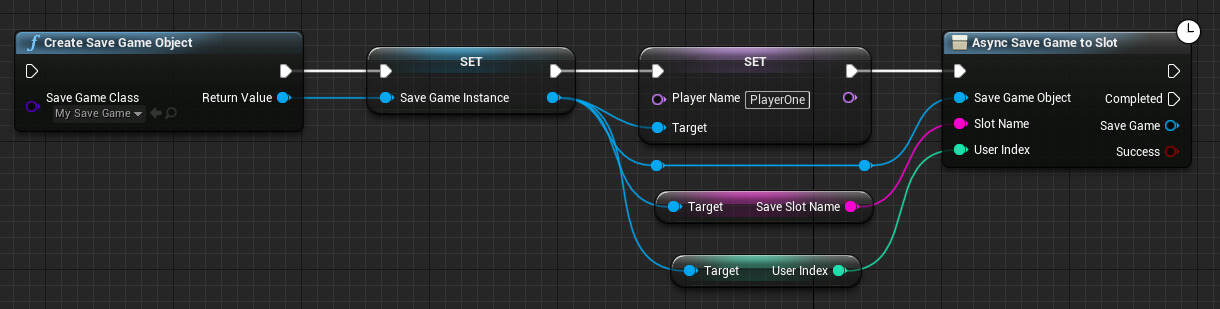
\includegraphics[width=1\textwidth]{images/SaveGameBP.png}
    \caption{Blueprint zum Speichern des Spielstandes mit der SaveGame-Klasse \cite{unrealengineSavingLoading}}
    \label{fig:unrealSaveGameBluePrintSave}
\end{figure}

Wie das Laden der Spieldaten mit der SaveGame-Klasse funktioniert, ist in dem Blueprint der Abbildung \ref{fig:unrealSaveGameBluePrintLoad} zu sehen. Zu Beginn wird der "Load Game from Slot"-Knoten gebraucht, um die Daten zu laden. Falls viele Daten geladen werden, oder es während der Ladezeit einen Lade-Bildschirm geben soll, wird auch hier von Epic Games der "Async Load Game from Slot"-Knoten empfohlen, der das Gleiche wie der "Load Game from Slot"-Knoten macht, aber asynchron arbeitet. Als Eingabe braucht dieser Knoten den Slot-Namen und den Benutzer-Index. Der Ausgabewert muss dann zur eigenen SaveGame-Klasse gecasted werden. Bei einem asynchronen Laden sollte zuerst mithilfe des "Is Valid"-Knotens überprüft werden, ob die Daten alle erfolgreich geladen wurden. Nach dem Cast zu der eigenen SaveGame-Klasse kann auf die Variablen dieser Klasse zugegriffen werden.\cite{unrealengineSavingLoading}

\begin{figure}[htp]
    \centering
    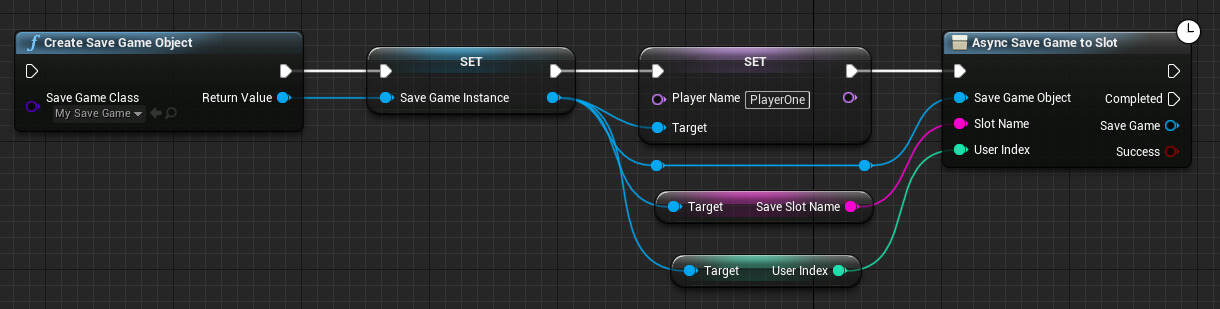
\includegraphics[width=1\textwidth]{images/SaveGameBP.png}
    \caption{Blueprint zum Laden des Spielstandes mit der SaveGame-Klasse \cite{unrealengineSavingLoading}}
    \label{fig:unrealSaveGameBluePrintLoad}
\end{figure}

Falls dieses Speicher- und Ladesystem in \cpp{}-Code geschrieben werden soll, muss die Header-Datei "Kismet/GameplayStatics.h" zu der eigenen SaveGame-Klasse hinzugefügt werden und diese muss dann als Kind-Klasse von der USaveGame-Klasse deklariert werden. In der eigenen SaveGame-Klasse können dann die zu speichernden Variablen, der Slot-Name und der Benutzer-Index definiert werden. Mithilfe der Funktion SaveGameToSlot oder AsyncSaveGameToSlot und LoadGameFromSlot oder AsyncLoadGameFromSlot aus der Klasse UGameplayStatics können die Daten synchron oder asynchron gespeichert und geladen werden.\cite{unrealengineSavingLoading}



\subsection{JSON}
Auch bei Unreal Engine ist es möglich, die Spieldaten im \ac{json}-Format abzuspeichern. Bei den Blueprints ist der Entwickler etwas eingeschränkt, da es erst seit Unreal Engine 5 Blueprints zum Arbeiten mit \ac{json} gibt und die Anzahl der Funktionen noch gering ist. Es gibt Knoten für Blueprints, bei denen ein \cpp{}-Struct zu einem \ac{json}-String umgewandelt wird, oder Knoten, bei denen bestimmte Schlüsselwerte von \ac{json}-Objekten zurückgegeben werden. Außerdem gibt es Knoten, die \ac{json}-Objekte aus Dateien speichern und laden können.\cite{unrealengineJsonBlueprint}

Mehr Möglichkeiten gibt es beim direkten Arbeiten mit \cpp{}, um zu \ac{json} zu serialisieren. Dafür gibt es zum Beispiel bei Unreal Engine eine \textit{FJsonSerializer-Klasse}.\cite{unrealengineFJsonSerializer} Zum Speichern der \ac{json}-Daten als \cpp{}-Objekt kann die \textit{FJsonObject-Klasse} verwendet werden.\cite{unrealengineFJsonObject} Zum Serialisieren und Deserialisieren wird dann der FJsonSerializer benutzt.\cite{unrealengineFJsonSerializer} In dem Listing \ref{lst:unrealFJsonSerializer} ist zu sehen, wie diese Klassen verwendet werden können. In den ersten vier Zeilen wird ein neues \ac{json}-Objekt erstellt, mit Schlüssel und Schlüsselwerten wie in dem Listing \ref{lst:jsonUtilityExp}. Danach wird in der Zeile 8 dieses \ac{json}-Objekt zu einem \ac{json}-String konvertiert und in dem Objekt "JsonString" gespeichert. In der Zeile 12 wird dieser String wieder deserialisiert und in einem \ac{json}-Objekt namens "JsonObject" gespeichert. Falls das Deserialisieren erfolgreich abläuft, ist die Kondition aus der Zeile 12 wahr und der Code in der Zeile 14 kann ausgeführt werden.\cite{wraiythUsingJson1}\cite{wraiythUsingJson2}

\begin{listing}[htp]
    \begin{minted}[breaklines,frame=single]{cpp}
        TSharedPtr JoeJsonObject = MakeShareable(new FJsonObject);
        JoeJsonObject->SetNumberField("level", 1);
        JoeJsonObject->SetNumberField("health", 75.2f);
        JoeJsonObject->SetStringField("name", "Joe");
        
        FString JsonString;
        TSharedRef<TJsonWriter<>> Writer = TJsonWriterFactory<>::Create(&JsonString);
        FJsonSerializer::Serialize(JoeJsonObject.ToSharedRef(), Writer);   
        
        TSharedPtr JsonObject;
        TSharedRef<TJsonReader<>> Reader = TJsonReaderFactory<>::Create(JsonString);
        if(FJsonSerializer::Deserialize(Reader, JsonObject)) 
        {
           ...
        }
    \end{minted}
    \caption{Serialisieren und Deserialisieren mit FJsonSerializer in Unreal Engine \cite{wraiythUsingJson1}\cite{wraiythUsingJson2}}
    \label{lst:unrealFJsonSerializer}
\end{listing}



\subsection{Save Extension}
Falls ein Entwickler ein fertiges Speicher- und Ladesystem sucht, welches er in sein Spiel integrieren möchte, dann ist \textit{Save Extension} geeignet. Dieses Plugin wurde für Unreal Engine 4 entwickelt und bietet eine Vielzahl an Funktionen an, die sowohl in \cpp{}-Code als auch als Blueprint implementiert werden können.\cite{unrealengineSaveExtension}

Die ersten Schritte zum Aufstellen des Speicher- und Ladesystems mit der Save Extension über ein Blueprint sind in der Abbildung \ref{fig:unrealSaveExtensionBlueprint} zu sehen. Die zwei Knoten "Save Slot to Id" und "Load Slot from Id" werden verwendet, um Daten aus einem bestimmten Slot zu speichern und zu laden. Jeder Slot kann eine bestimmte Spielwelt von einem Spieler sein und wird in einer eigenen Datei gespeichert.\cite{piperiftPiperiftSaveSlot} Um einen bestimmten Slot auszuwählen, gibt es die Eingabe "Slot Id", in der die Slot-Nummer eingegeben werden kann. Beim Speichern kann auch ausgewählt werden, ob der alte Spielstand eines Slots überschrieben werden soll, falls einer existiert. Zum Auslösen des Speicherns oder Ladens gibt es einige Möglichkeiten. In der Abbildung \ref{fig:unrealSaveExtensionBlueprint} zum Beispiel wird das Speichern des Spielstandes dadurch ausgelöst, dass die Taste K gedrückt wurde. Zum Laden muss in diesem Beispiel die Taste L gedrückt werden. Alternativ unterstützt das Save Extension-Plugin auch ein Auto-Save und Auto-Load. Beim Auto-Save wird automatisch der aktuelle Slot gespeichert und beim Auto-Load wird immer der letzte aktive Slot geladen. Ein Slot wird als aktiv markiert, wenn er geladen wird.\cite{piperiftPiperiftSaveSlot}\cite{piperiftPiperiftSaveBlueprint} 

\begin{figure}[htp]
    \centering
    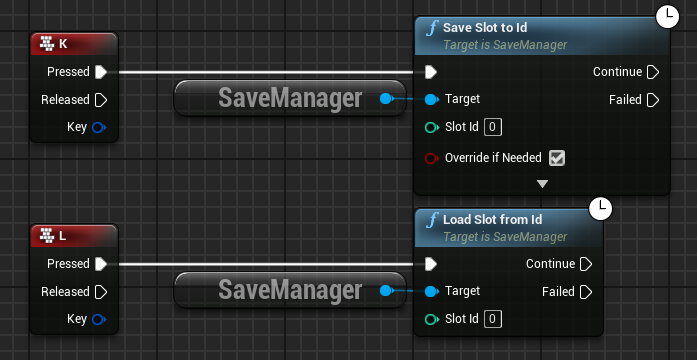
\includegraphics[width=0.8\textwidth]{images/SaveExtension_load_save_blueprint.png}
    \caption{Blueprint zum Laden der Daten mit dem Save Extension-Plugin \cite{piperiftPiperiftSaveBlueprint}}
    \label{fig:unrealSaveExtensionBlueprint}
\end{figure}

Nach dieser Einrichtung werden noch keine Actor\footnote{Actors sind bei Unreal Engine alle Spielobjekte, die in die Spielwelt geladen werden.\cite{unrealengineActors}}-Klassen oder Components\footnote{Components werden an Actors angehängt und beeinflussen, wie sich diese verhalten.\cite{unrealengineActors}} gespeichert. Über das \textit{SavePreset} Blueprint lassen sich Actors und Component-Klassen zum Speicher- und Ladesystem hinzufügen. Um dann Variablen eines Actors oder Components abzuspeichern, muss für jede zu speichernde Variable die "SaveGame"-Eigenschaften angeklickt werden. Komprimierung der Daten ist bei der Save Extension auch möglich. Dies kann bei dem SavePreset eingestellt werden.

Um zu vermeiden, dass zu viele Daten geladen werden, werden Slots in zwei Bereiche unterteilt und gespeichert. Es gibt einmal die Slot Info, die leichtgewichtete Daten über die Spielwelt speichert. Diese enthält zum Beispiel das Level des Spielers, seinen Spielername oder in welchem Bereich der Spielwelt sich der Spieler bei dem Spielstand befindet. Der Rest wird im "Slot Data"-Bereich gespeichert. Hier sind alle Informationen der serialisierten Actors und Components der Spielwelt eines Slots. Diese Unterteilung ist praktisch, wenn wenige Slot-Informationen benötigt werden, aber diese nicht komplett geladen werden sollen. Falls zum Beispiel ein Menü erstellt wird, wo ausgewählt werden kann, mit welcher Spielwelt weitergespielt werden soll, kann hier bei jeder Spielwelt ein paar Informationen über diese beschrieben werden, ohne alle Slots komplett zu laden.\cite{piperiftPiperiftSaveSlot}

Eine weitere Funktion, die die Effizienz des Speicherns enorm verbessern kann, ist die Möglichkeit, asynchron zu arbeiten. Bei dem Save Extension-Plugin gibt es einmal die Multithreaded oder Frame-splitted Serialisierung, bei der die zu serialisierenden Daten auf alle verfügbaren CPU-Threads oder auf mehrere Frames verteilt und dort einzeln serialisiert werden. Außerdem gibt es noch Multithreaded-Dateien, die asynchron im Hintergrund der Anwendung komprimiert, gespeichert und geladen werden.\cite{piperiftPiperiftSaveMultithreaded}

Der Speicherprozess besteht aus den folgenden Schritten: Als Erstes wird der alte Spielstand gelöscht und es wird die Funktion OnSaveBegan aufgerufen, um weiterzugeben, dass der Speicherprozess begonnen hat. Dann werden der Thumbnail des aktuellen Spieles und die Spielstatistiken abgespeichert und anschließend wird die Spielwelt serialisiert. Zum Schluss wird die Funktion OnSaveFinished aufgerufen, um weiterzugeben, dass der Speicherprozess beendet wurde. In der Abbildung \ref{fig:piperiftSaveProcess} ist der vollständige Speicherprozess zu sehen. Gestrichelte Kanten bedeuten, dass hier mehrere Prozesse parallel laufen können.\cite{piperiftSaveProcess}

\begin{figure}[htp]
    \centering
    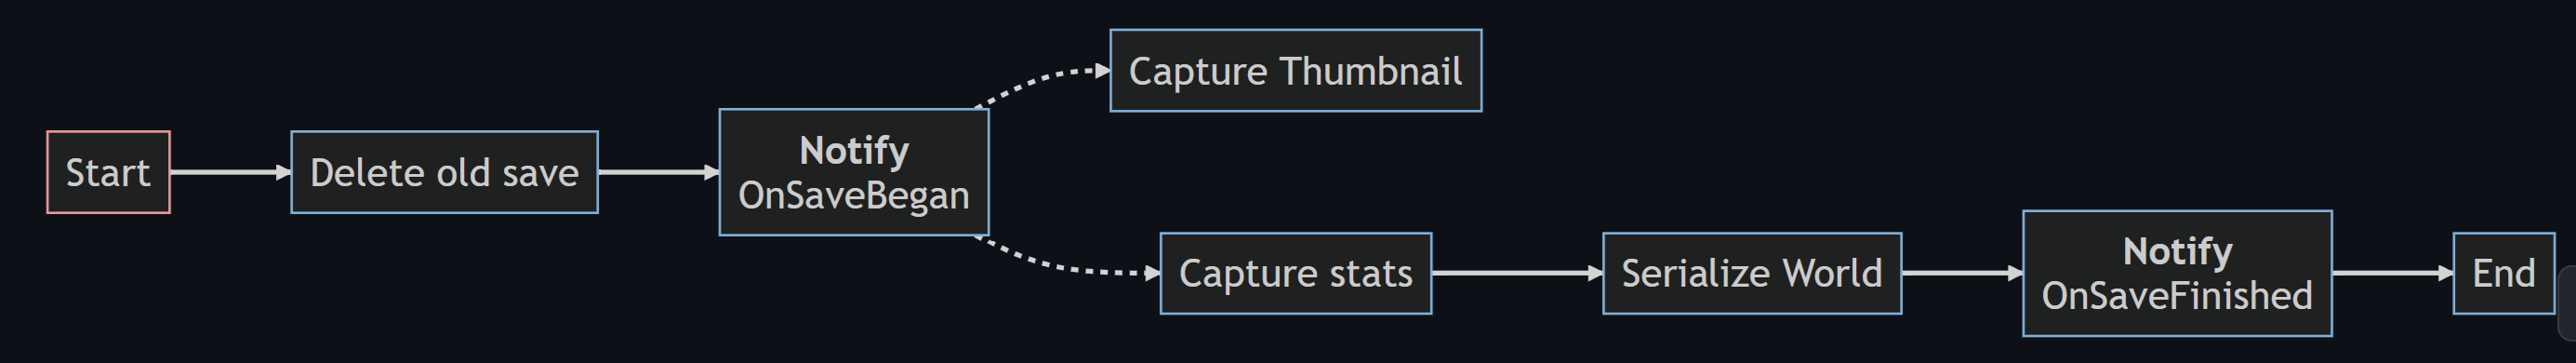
\includegraphics[width=1\textwidth]{images/piperift_save_process.png}
    \caption{Speicherprozess des Save Extension-Plugins \cite{piperiftSaveProcess}}
    \label{fig:piperiftSaveProcess}
\end{figure}

Der Ladeprozess ist etwas komplexer. Als Erstes wird die Funktion OnLoadBegan aufgerufen, um den Start des Ladeprozesses weiterzugeben. Danach werden alle Maps und Daten geladen und anschließend werden die Filter der einzelnen Level und generelle Filter vorbereitet, damit überprüft werden kann, welcher Actor in welchem Level geladen werden muss und wie dieser deserialisiert werden soll. Hiernach werden die einzelnen Levels vorbereitet und die Welt wird deserialisiert. Beim Vorbereiten der Levels werden gespeicherte Actors wiederhergestellt und nicht mehr existierende endgültig gelöscht. Beim Deserialisieren der Welt werden alle Level abgearbeitet und deren Actors und Components deserialisiert. Zum Schluss wird die Funktion OnLoadFinished aufgerufen, um weiterzugeben, dass der Ladeprozess terminiert hat. In der Abbildung \ref{fig:piperiftLoadProcess} ist der vollständige Ladeprozess zu sehen.\cite{piperiftLoadProcess}

\begin{figure}[htp]
    \centering
    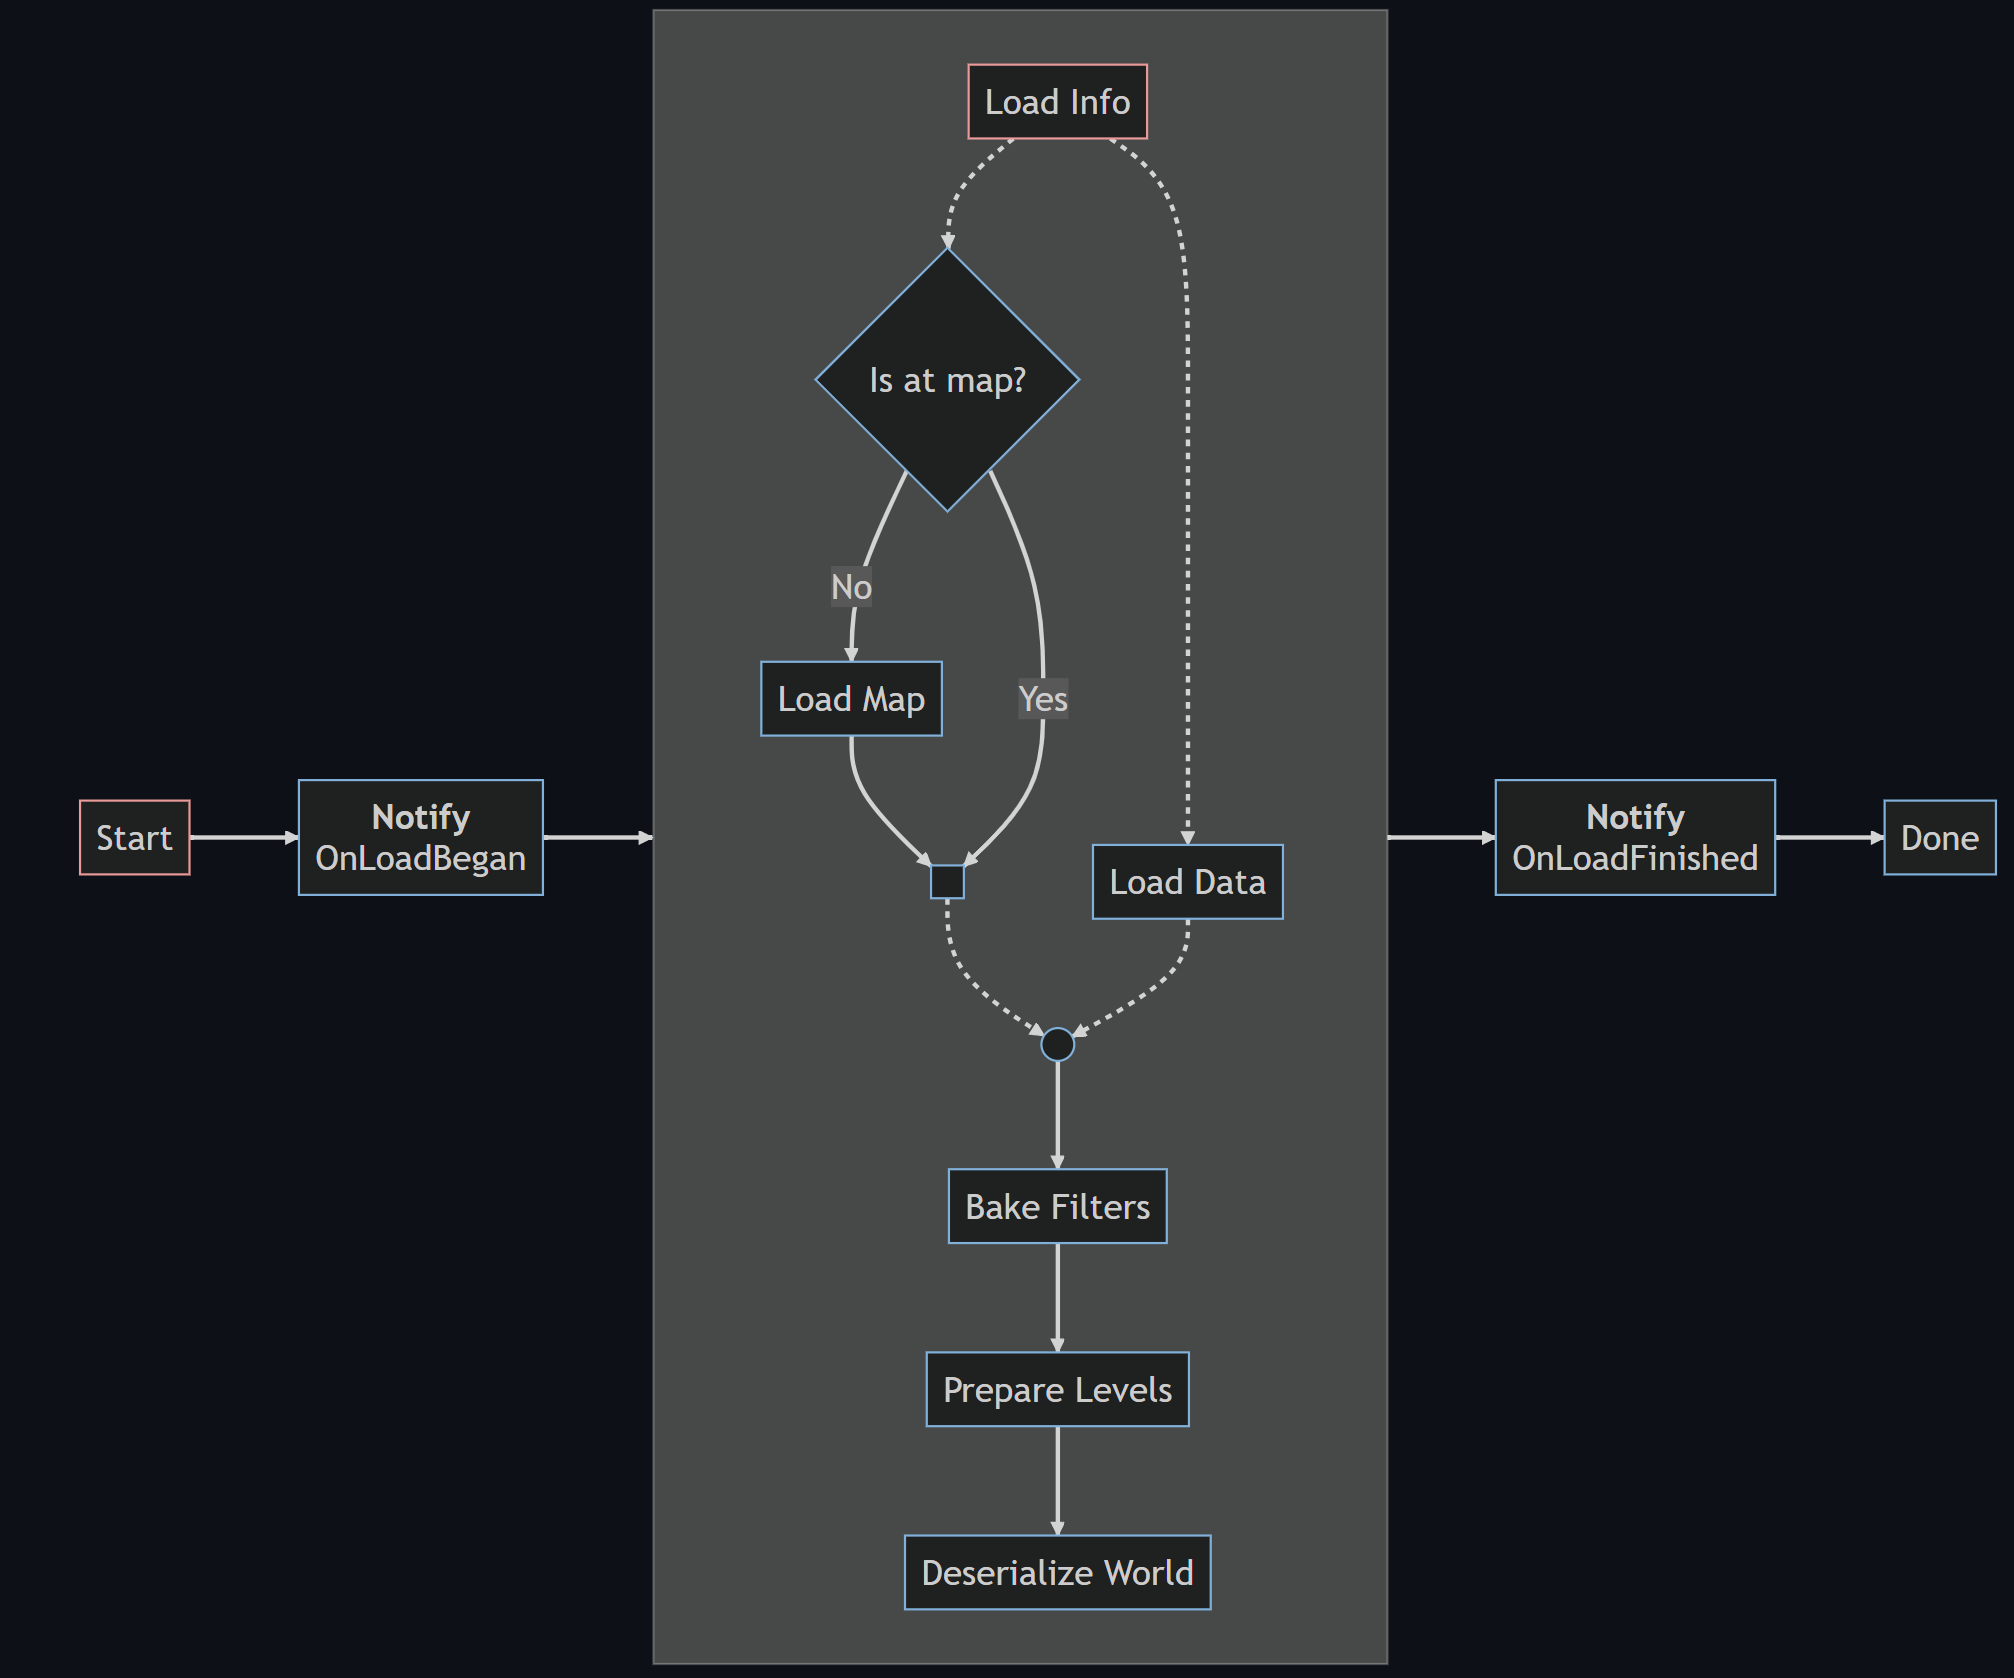
\includegraphics[width=0.8\textwidth]{images/piperift_load_process.png}
    \caption{Ladeprozess des Save Extension-Plugins \cite{piperiftLoadProcess}}
    \label{fig:piperiftLoadProcess}
\end{figure}



\subsection{Strategie für Unreal Engine}
Auch bei Unreal Engine gibt es keine beste Lösung für das Speichern und Laden von Spielständen. Bei den von Unreal Engine bereitgestellten Tools eignet sich am besten die SaveGame-Klasse. Diese wird von Epic Games empfohlen, wenn ein Speicher- und Ladesystem aufgebaut werden muss. Die Serialisierung zu \ac{json} über die Blueprints, die schon in Unreal Engine eingebaut sind, scheint umständlich zu sein, da sie wenige Funktionen anbietet. 

Falls das System ohne Problem auf mehr Daten erweitert werden soll, wird das Arbeiten mit Blueprints ein großer Aufwand. Bei vielen Daten, die gespeichert werden sollen, wird es schnell unübersichtlich mit der graphischen Oberfläche der Blueprints. Es gestaltet sich schwierig, eine klare Übersicht darüber zu gewinnen, welche Knoten mit welchen verbunden sind. Außerdem wird fortgeschrittenen Entwicklern empfohlen, \cpp{} zu verwenden, da damit effizientere Algorithmen als mit den Blueprints entwickelt werden können.\cite{epicgamesComparingBlueprints} Als Alternative zu der Blueprint-Strategie kann die FJsonSerializer- oder SaveGame-Klasse von Unreal Engine verwendet werden. Welche Option geeigneter ist, hängt auch von den Präferenzen des Entwicklers ab. Falls die Daten im \ac{json}-Format gespeichert werden müssen, ist die FJsonSerializer-Klasse angebrachter. Ansonsten kann auch hier die von Epic Games empfohlene SaveGame-Klasse verwendet werden, um mit \cpp{}-Code die Daten zu speichern.

Auch bei Unreal Engine kann ein fertiges Speicher- und Ladesystem verwendet werden, falls der Entwickler möglichst viel Zeit sparen möchte. Die Save Extension ist eine gute Alternative zu den von Epic Games bereitgestellten Tools. Sie ist kostenfrei und bietet einige Möglichkeiten an, den Speicher- und Ladeprozess zu beschleunigen. 
%--------------------------------------------------------------------------



%--------------------------------------------------------------------------
\section{Godot}
Die Godot Engine ist eine kostenlose open-source Game Engine, welches von einer Gemeinschaft von unabhängigen Entwicklern erstellt wurde. Sie wurde 2014 veröffentlicht und wird hauptsächlich für kleinere Spiele verwendet, da es im Vergleich zu anderen Game Engines weniger Funktionen bereitstellt. Im Vergleich zu Unity und Unreal Engine verwendet Godot keinen komponentenbasierten Ansatz, sondern hat verschiedene Klassen von Objekten, die Nodes genannt werden. Diese werden in einer Hierarchie in der Spiel-Szene angeordnet und jedem Node kann ein Skript angehängt werden, um dessen Verhalten anzupassen. Statt bereits existierende Programmiersprachen zu verwenden, wurde für Godot eine eigene Programmiersprache entwickelt, namens GDScript, welche viele Ähnlichkeiten zu Python besitzt. Alternativ können aber auch \csharp{} und \cpp{} verwendet werden. Mit der Godot Engine können 2D- und 3D-Spiele für Desktop-Plattformen, Mobilgeräte und das Web entwickelt werden.\cite{salmela2022game}

Zu Beginn von diesem Abschnitt werden zwei Möglichkeiten betrachtet, die von Godot Engine angeboten werden, um Spielobjekte zu serialisieren und deserialisieren. Einmal wird das Arbeiten mit \ac{json} betrachtet und danach die binäre Serialisierung. Zum Schluss wird noch ein Godot-Plugin vorgestellt, welches ein fertiges Speicher- und Ladesystem für Entwickler anbietet. 



\subsection{JSON}
Da die Programmiersprache GDScript Dictionaries unterstützt, ist es sinnvoll, mit \ac{json} zu arbeiten, da diese im GDScript bereits eine sehr \ac{json}-ähnliche Struktur besitzen. Um ein Speicher- und Ladesystem mit Godot Engine im \ac{json}-Format aufzustellen, sollten zu Beginn erst einmal alle Objekte, die gespeichert werden sollen, markiert werden. Jedes Objekt kann zu einer Gruppe hinzugefügt werden. Gruppen sind Ansammlungen von Objekten mit einem bestimmten Namen, wobei jedes Objekt auch mehreren Gruppen zugehören kann. Danach muss zu allen Objekten, die gespeichert werden sollen, eine Funktion hinzugefügt werden, die das Objekt zu einem \ac{json}-Objekt umwandelt. Wie so eine Funktion aussehen kann, ist in dem Listing \ref{lst:godotJsonToJsonFunc} zu sehen. Alle wichtigen Variablen eines Objektes werden in ein Dictionary gespeichert und danach mithilfe der "\ac{json}"-Hilfsklasse zu einem \ac{json}-String umgewandelt. Diese Klasse hat aber auch Einschränkungen, was alles in \ac{json} umgewandelt werden kann. Zum Beispiel können Vektoren, wie der "position"-Vektor eines Objektes, nicht direkt in \ac{json} umgewandelt werden. Deshalb muss die Position über eine x- und y-Variable gespeichert werden, statt direkt den "position"-Vektor zu speichern.\cite{godotengineSavingGames}

\begin{listing}[htp]
    \begin{minted}[breaklines,frame=single,tabsize=2]{python}
        func to_json():
          var object_data = {
            "filename" : get_scene_file_path(),
            "parent" : get_parent().get_path(),
            "x" : position.x, 
            "y" : position.y,
            "level": level,
            "health": health,
            "name": name
          }

          return JSON.stringify(object_data)
    \end{minted}
    \caption{Konvertierung der zu speichernden Klassendaten zu \ac{json} in Godot \cite{godotengineSavingGames}}
    \label{lst:godotJsonToJsonFunc}
\end{listing}

Die "to\_json"-Funktion kann zum Speichern aller Objektzustände verwendet werden. In dem Code \ref{lst:godotJsonSave} ist zu sehen, wie eine Speicherfunktion aussehen könnte. Dabei wird als Erstes eine Datei definiert, in der die Daten gespeichert werden sollen. Danach werden alle Objekte aus der "Save"-Gruppe geholt und über diese Menge wird iteriert. Wenn ein Objekt gespeichert werden soll, muss es zu dieser Gruppe hinzugefügt werden. Für jedes Objekt dieser Gruppe wird erst einmal geschaut, ob dieses Objekt aus einer Datei instanziiert wurde und ob in diesem Objekt die "to\_json"-Funktion enthalten ist. Nodes bei Godot haben immer die Variable "scene\_file\_path", welche als String speichert, aus welcher Datei das Objekt instanziiert wurde. Alle Kind-Nodes dieses Objektes haben bei dieser Variable einen leeren String.\cite{godotengineNode} Diese Nodes sollen beim Speichern übersprungen werden. Bei den restlichen Objekten wird die "to\_json"-Funktion aufgerufen und der \ac{json}-String, der zurückgegeben wird, wird in die Speicherdatei geschrieben.\cite{godotengineSavingGames} Falls sich ein Dateiname der Objekte verändern sollte, weil der Entwickler diese zum Beispiel geändert hat, müssen alle Spielstände angepasst werden, da ansonsten die Datei der Objekte nicht gefunden werden kann.

\begin{listing}[htp]
    \begin{minted}[breaklines,frame=single]{python}
        func save_game():
          var save_game = FileAccess.open("user://savegame.save", FileAccess.WRITE)
          var save_nodes = get_tree().get_nodes_in_group("Save")
          for node in save_nodes:
            if node.scene_file_path.is_empty() || !node.has_method("to_json"): 
              continue 

            var json_string = node.call("to_json")
            save_game.store_line(json_string)
    \end{minted}
    \caption{Speichern aller JSON-Daten der Knoten aus der "Save"-Gruppe \cite{godotengineSavingGames}}
    \label{lst:godotJsonSave}
\end{listing}

Im Vergleich zum Speichern müssen beim Laden der Daten mehr Schritte durchgeführt werden. In dem Code \ref{lst:godotJsonLoad} ist zu sehen, wie ein Spiel in Godot über eine "load\_game"-Funktion geladen werden kann, abhängig von den letzten zwei GDScripts. Zu Beginn sollte überprüft werden, ob die Speicherdatei existiert. Wenn das der Fall ist, kann der Prozess fortgesetzt werden. Als nächstes wird geschaut, ob bereits Objekte der "Save"-Group existieren. Diese müssen gelöscht werden, weil sonst beim Laden Duplikate entstehen könnten. Danach kann begonnen werden, die Speicherdatei Zeile für Zeile abzulesen. Da die Objekte immer als einzeilige \ac{json}-Strings gespeichert werden, stellt jede Zeile in der Speicherdatei ein Objekt dar. Dieses \ac{json}-Objekt wird dann über die "parse"-Funktion der \ac{json}-Hilfsklasse deserialisiert. Falls das Deserialisieren erfolgreich war, werden die Daten des Objektes an die "load\_node"-Funktion weitergegeben. Diese instanziiert das Objekt und setzt die Werte der gespeicherten Variablen.\cite{godotengineSavingGames}

\begin{listing}[htp]
    \begin{minted}[breaklines,frame=single]{python}
        func load_game():
          if not FileAccess.file_exists("user://savegame.save"):
            return

          var save_nodes = get_tree().get_nodes_in_group("Save")
          for i in save_nodes:
            i.queue_free()

          var save_game = FileAccess.open("user://savegame.save", FileAccess.READ)
          while save_game.get_position() < save_game.get_length():
            var json_string = save_game.get_line()
            var json = JSON.new()

            var parse_result = json.parse(json_string)
            if not parse_result == OK: continue

            load_node(json.get_data())

        func load_node(node_data):
          var new_object = load(node_data["filename"]).instantiate()
          get_node(node_data["parent"]).add_child(new_object)
          new_object.position = Vector2(node_data["x"], node_data["y"])

          for key in node_data.keys():
            if key == "filename" or key == "parent" or key == "x" or key == "y":
              continue
            new_object.set(i, node_data[i])
    \end{minted}
    \caption{Laden der in \ref{lst:godotJsonSave} gespeicherten Daten \cite{godotengineSavingGames}}
    \label{lst:godotJsonLoad}
\end{listing} 



\subsection{Binary Serialization}
Auch binäre Serialisierung wird von Godot unterstützt. Bei diesem Prozess werden die verschiedenen Datentypen zu einem Array von Bytes umgewandelt. Von Godot Engine werden 30 verschiedene Datentypen\cite{godotengineBinarySerialization} bereitgestellt, die im binären Format gespeichert werden können. Beim Serialisieren werden die Daten in Pakete verpackt. Ein Paket ist ein Datentyp mit seinem Wert. Die ersten vier Bytes eines Pakets beschreiben den Datentypen und werden zum Setzen von Flags verwendet. Jeder Datentyp ist als Zahl definiert, welche im Header binär geschrieben wird. Zum Beispiel ist der Datentyp "int" mit der Zahl 2 definiert und über Flags kann gespeichert werden, ob es ein 32-Bit- oder 64-Bit-Integer ist. Ab dem fünften Byte beginnt der Inhalt des Pakets. Dieser variiert von Datentyp zu Datentyp. Bei Strings zum Beispiel wird in den ersten vier Bytes des Inhalts definiert, wie lang die Zeichenkette ist, und erst nach diesen vier Bytes wird der String-Inhalt bestimmt. Bei solchen Datentypen ist die Größe des Paketinhalts variabel und nicht fest definiert.\cite{godotengineBinarySerialization}

Objekte können über Godots "var\_to\_bytes\_with\_objects"-Funktion binär serialisiert und mit der "bytes\_to\_var\_with\_objects"-Funktion wieder deserialisiert werden. Beim Deserialisieren muss jedoch beachtet werden, dass die Daten keinen Code beinhalten, der ausgeführt werden kann. Es sollten immer nur Daten von vertrauten Quellen deserialisiert werden, sonst können Probleme entstehen, die bei dem BinaryFormatter-Abschnitt \ref{ssec:binaryFormatter} genauer beschrieben wurden.\cite{godotengineGlobalScope}

Die binäre Serialisierung hat viele Vorteile gegenüber der \ac{json}-Serialisierung. Zum einen sind die Dateigrößen deutlich kompakter bei binären Daten, im Vergleich zu den gespeicherten \ac{json}-Strings. Zum anderen unterstützt Godot viel mehr Datentypen, die binär, aber nicht zu \ac{json} serialisiert werden können. Bei eigenen Klassen braucht es auch eigene Logik zum Kodieren und Dekodieren dieser, um das Serialisieren zu \ac{json} zu ermöglichen. Bei binärer Serialisierung wird weniger eigene Logik benötigt.\cite{godotengineSavingGames}



\subsection{Thoth}
Falls ein fertiges Speicher- und Ladesystem gesucht wird, welches in das Projekt integriert werden soll, dann ist das Plugin \textit{Thoth} eine Alternative zu den eingebauten Godot Engine-Funktionen. Dieses System wurde so entwickelt, dass es für jede Art von Spiel verwendet werden kann und speichert den Spielzustand in einem Format, welches ähnlich zu \ac{json} ist.\cite{stupidratstudioGodotSaveLoad}

Um das System aufzustellen, muss das "Savestate"-Node von diesem Plugin hinzugefügt werden. Diese Node ist immer mit einer Speicherdatei verbunden und kann den Spielzustand zu einem beliebigen Zeitpunkt speichern. Im GDScript-Listing \ref{lst:godotThoth} ist zu sehen, wie das "Savestate"-Node verwendet werden kann. Als Erstes wird in dem Array "serializable\_collections" definiert, welche Objekte serialisiert werden sollen. In dem Beispielcode werden alle Kinder-Nodes von dem "SaveObjects"-Node serialisiert. Bei jedem Objekt kann außerdem mit dem "serializable"-Array eingestellt werden, welche Variable gespeichert wird. In dem Objekt, zu dem der Code aus dem Listing \ref{lst:godotThothObject} gehört, werden zum Beispiel nur die Variablen "level", "health" und "name" gespeichert. Die Variable "effects" wird beim Serialisieren übersprungen. Zum Speichern und Laden müssen die Funktionen "save\_game" und "load\_game" aus dem Listing \ref{lst:godotThoth} aufgerufen werden. Bei der Speicherfunktion müssen als Erstes die gespeicherten Daten geladen werden, da es möglich ist, dass noch Informationen der alten Spielstände gebraucht werden. Anschließend kann der aktuelle Spielzustand serialisiert und dann gespeichert werden. Bei der Ladefunktion wird als Erstes der letzte Spielzustand geladen und danach deserialisiert.\cite{stupidratstudioGodotSaveLoad} 

\begin{listing}[htp]
    \begin{minted}[breaklines,frame=single]{python}
        extends Node2D

        const serializable_collections = [
          "SaveObjects"
        ]

        @onready var savestate = get_node("Savestate")

        func save_game():
          savestate.load_game_state()
          savestate.pack_game_state(self)  
          savestate.save_game_state()

        func load_game():
          savestate.load_game_state()
          savestate.unpack_game_state(self)
    \end{minted}
    \caption{Speichern und Laden des "SaveObjects"-Knoten mit Thoth \cite{stupidratstudioGodotSaveLoad}}
    \label{lst:godotThoth}
\end{listing} 

\begin{listing}[htp]
    \begin{minted}[breaklines,frame=single]{python}
        extends Node2D

        var level
        var health
        var name
        var effects

        const serializable = [
            "level",
            "health",
            "name"
        ]

        ...
    \end{minted}
    \caption{Thoth-Einstellung, welche Variablen einer Klasse serialisiert werden sollen \cite{stupidratstudioGodotSaveLoad}}
    \label{lst:godotThothObject}
\end{listing} 



\subsection{Strategie für Godot Engine}
Auch bei Godot gibt es keine Strategie, die beim Speichern und Laden des Spielstandes vorteilhafter ist als alle andere. Auch bei Godot ist dies abhängig vom Anwendungsfall. Falls das Speicher- und Ladesystem selber vom Entwickler komplett implementiert werden soll, eignet es sich, mit den eingebauten Tools von Godot Engine zu arbeiten. Hier hat die binäre Serialisierung auch mehr Vorteile. Sie ist schneller, die Daten sind kompakter und es werden deutlich mehr Datentypen unterstützt, wodurch der Entwickler weniger eigenen Code zum Serialisieren und Deserialisieren der Daten schreiben muss. Die einzigen Gründe, stattdessen die \ac{json}-Hilfsklasse zu verwenden, sind, dass die gespeicherten Daten im binären Format nicht von Menschen gelesen werden können und dass Veränderungen der Datenstruktur zu Problemen führen können. Wenn es dazu kommt, muss der Entwickler alle Daten selber auf die neue Datenstruktur anpassen. Falls die Lesbarkeit wichtig ist und sich die Datenstrukturen des Öfteren verändern könnten, sollte mit \ac{json} gearbeitet werden.

Auch bei Godot hat ein Entwickler die Möglichkeit, Zeit durch das Verwenden eines fertigen Speicher- und Ladesystems zu sparen. Hier kann zum Beispiel Thoth verwendet werden, mit dem das System in wenigen Schritten implementiert werden kann. Da als Entwickler noch einige Zeilen Code geschrieben werden müssen, bei denen verschiedene Funktionen von Thoth aufgerufen werden, gibt es noch einige Möglichkeiten, das System anzupassen und gegebenenfalls zu optimieren.